%% -*- eval: (flyspell-mode 1); -*-

\chapter{\'Evaluation de la bibliothèque}

Le DSEL doit être évalué dans plusieurs domaines : à la fois du point de vue de l'expressivité du langage et du point de vue des performances obtenues (la rapidité d'exécution). Ces deux évaluations ont été difficiles à réaliser car d'une part l'expressivité est difficilement quantifiable, et d'autre part le DSEL s'appuie sur la bibliothèque \textsf{triSYCL} qui est seulement un prototype dont l'objectif principal n'est pas la performance mais la preuve de faisabilité.


\section{\'Evaluation qualitative}

La qualité du DSEL peut se juger à la facilité d'écriture de code l'utilisant. Globalement il faudrait alors évaluer à quel point la librairie permet d'abstraire le problème qu'elle est censée résoudre (ici la parallélisation de stencils). Plus particulièrement il s'agit de quantifier notamment le pseudo-typage (comme la détection statique d'erreurs sémantiques), le nombre de mots-clés (classes, méthodes), le nombre de symboles, et enfin le nombre de lignes de codes (LOC). Pour des raisons de simplicité seul le nombre de ligne de codes ainsi que le nombre de caractères ont été pris en compte. 

Ces deux nombres ont été comparés entre plusieurs codes d'un même problème de Jacobi en deux dimensions avec un stencil à cinq points. Les différentes versions comparées sont :
\begin{enumerate}
\item code de base sans parallélisation ;
\item code \textsf{OpenMP} avec parallélisation naïve ;
\item code \textsf{OpenMP} avec parallélisation par tuilage ;
\item code \textsf{triSYCL} avec parallélisation naïve ;
\item code \textsf{triSYCL} avec parallélisation par tuilage ;
\item code \textsf{DSEL} avec parallélisation et coefficients variables ;
\item code \textsf{DSEL} avec parallélisation et coefficients constants ;
\item code \textsf{OpenCL} avec parallélisation par tuilage.
\end{enumerate}

Les deux versions du DSEL ne se déclinent pas en parallélisation avec tuilage ou naïve puisque celle-ci est simplement choisie par l'appel d'une méthode ou l'autre, dont les noms ne diffèrent que de cinq caractères (qui ont été comptabilisés). Par ailleurs pour comptabiliser les lignes de codes et caractères, toutes les lignes vides sont exclues, de même que les commentaires. De plus les conventions de codage (pour les retours à la ligne et la disposition des arguments) sont les mêmes pour les huit codes. Enfin aucune entrée/sortie standard (en dehors des erreurs) n'est intégrée dans le décompte des deux métriques. Les seules erreurs reportées se trouvent dans le code d'\textsf{OpenCL}, car c'est à la charge de l'utilisateur de les traiter contrairement aux autres codes. En effet (\textsf{OpenMP} n'en a pas besoin dans ce cas, et celles de \textsf{triSYCL} sont gérées en interne de même que le DSEL qui s'appuie sur \textsf{triSYCL}).

Les résultats sont reproduits dans le tableau \ref{tab:eval_qual} où l'on peut observer que le DSEL (avec coefficients constants) est le troisième code le plus court avec $42$ lignes, tandis que le plus court (code de base) en comporte $31$. Le DSEL avec coefficients constants se classe cinquième avec $46$ lignes. En ce qui concerne les codes avec tuilage, ils sont deux fois (\textsf{OpenMP}) à cinq fois (\textsf{OpenCL}) plus longs que le code de base. Le classement est quasiment identique selon le nombre de caractères (à une inversion près, ne concernant pas le DSEL).

\begin{table}
\floatbox[{\capbeside\thisfloatsetup{capbesideposition={right,center},capbesidewidth=4cm}}]{table}[\FBwidth]
{
\caption{Évaluation du nombre de lignes de codes et de caractères pour différentes implantations d'un problème Jacobi2D.}
\label{tab:eval_qual}
}
{
\begin{tabular}{||c||c|c||}
\hline
implantation & LOCs & caractères \\
\hline
\hline
base & $31$ & $899$ \\
\hline
OpenMP naïf & $32$ & $924$ \\
\hline
OpenMP tuilage & $87$ & $3115$ \\
\hline
triSYCL naïf & $43$ & $1676$ \\
\hline
triSYCL tuilage & $74$ & $3647$ \\
\hline
DSEL variable & $46$ & $1919$ \\
\hline
DSEL constant & $42$ & $1624$ \\
\hline
OpenCL tuilage & $177$ & $6266$ \\
\hline
\end{tabular}
}
\end{table}

En résumé, l'écriture du code grâce au DSEL est du même ordre de grandeur que l'écriture des codes parallélisés naïfs (à quelques lignes près supplémentaires) alors qu'il propose l'optimisation de tuilage. Les autres codes proposant le tuilage étant quant à eux deux à cinq fois plus longs que le code de base, le DSEL permet ainsi une amélioration significative des performances (grâce au tuilage) sans augmenter substantiellement la charge de développement (estimée en LOCs).


\section{Performances quantitatives sur machines dédiées}

Les performances quantitatives s'appuient sur deux métriques : le temps d'exécution et les compteurs \emph{hardwares}. Tandis que la rapidité d'exécution est l'objectif principal de la librairie, les compteurs permettent de comptabiliser indirectement la réutilisation des données, qui, plus elle est élevée plus elle favorise la rapidité. Le protocole de tests est présenté en premier, avant de préciser plus en détail les résultats de ces mesures.

\subsection{Description du matériel et des cas de tests}
\label{sec:desc_mat_tests}

L'optimisation des calculs faisant intervenir de nombreux paramètres, plusieurs implantations et machines différentes ont été utilisées. Le protocole de test consiste à exécuter chacune des implantations deux ou trois fois de suite (selon les machines) pour un même jeu de paramètres, puis de faire varier ces paramètres et recommencer. C'est la moyenne des résultats des deux ou trois exécutions de chaque cas de test qui est ici analysée, ce faible nombre d'exécutions est suffisant puisque les premières mesures manuelles n'ont révélé que des différences entre elles inférieures à $1\%$. Par ailleurs chaque implantation applique trois fois le stencil d'affilée, les résultats des mesures de chacune des trois applications sont simplement sommés formant alors le résultat utilisé pour calculer la moyenne.

\subsubsection*{Implantations testées}

Afin de pouvoir évaluer certains paramètres pouvant influencer les performances, il a été nécessaire de ne pas utiliser directement le DSEL produit mais uniquement la bibliothèque \textsf{triSYCL} de parallélisation sur laquelle il s'appuie ainsi qu'\textsf{OpenMP} (utilisée par \textsf{triSYCL}). Toutefois cela n'a pas d'impact sur les performances, car les implantations ont été écrites dans l'esprit du code automatique produit par le DSEL. De plus les méthodes du DSEL sont marquées pour être \emph{inlinées} dans le code d'origine, et ne provoquent donc pas d'appels supplémentaires dans l'exécution du programme. Ainsi nous pouvons considérer que les performances mesurées sont équivalentes à celles du DSEL.

Ne pas utiliser directement le DSEL permet notamment de modifier artificiellement le coût du calcul d'un élément de la grille dans le problème de Jacobi en deux dimensions. En effet chaque élément de la grille est dupliqué un certain nombre de fois (paramètre variable), la charge de calcul est donc dupliquée autant de fois. En pratique chaque élément représente donc une \emph{tuile} dont tous les sous-éléments sont identiques. L'application d'un coefficient sur un élément correspond alors à la multiplication matricielle de la tuile (qui est un vecteur à une seule dimension) par une matrice identité dont la diagonale a la valeur du coefficient originel. Moduler le coût du calcul d'un élément permet à la fois de modifier sa durée, et aussi la quantité de mémoire qu'il utilise puisque l'élément est dupliqué.

Afin de vérifier que l'implantation elle-même est valide, une vérification automatique des résultats a été réalisée dans le problème d'origine, sans tuile. En revanche les implantations évaluées dont les résultats sont présentés dans les sections suivantes ne concernent que des implantations avec tuiles. Elles ne nécessitent que quelques lignes de code supplémentaires mais ralentissent énormément la vérification des résultats (puisque chaque élément est dupliqué un certain nombre de fois) ; ainsi seule une vérification manuelle a été faite sur des petits jeux de données. Par ailleurs l'application du stencil est volontairement divergente afin de pouvoir distinguer les valeurs des éléments avant et après l'application du stencil. Ces vérifications n'ont pas permis de détecter une erreur significative (à $1^{-06}$ près) entre les différentes implantations, que nous considérons donc valides. 

Seuls deux paramètres de tests ont été étudiés :
\begin{itemize}
\item la taille de chaque macro-tuile carrée ;
\item la taille de chaque tuile.
\end{itemize}
Les autres paramètres n'ont pas été étudiés soit par manque de temps, soit parce qu'ils n'ont pas d'influence a priori (telle que la taille globale du système que nous supposons toujours inférieure à la taille de la RAM).

Ces deux paramètres peuvent alors influencer le comportement des implantations suivantes testées :
\begin{enumerate}
\item parallélisation naïve par \textsf{OpenMP} ;
\item parallélisation naïve par \textsf{triSYCL} (qui s'appuie sur \textsf{OpenMP}) ;
\item parallélisation par tuilage avec \textsf{OpenMP} ;
%% \item parallélisation par tuilage en column major avec \textsf{OpenMP} ;
\item parallélisation par tuilage avec \textsf{OpenMP}, représentation des macro-tuiles continue en mémoire RAM ;
\item parallélisation par tuilage avec \textsf{OpenMP}, parallélisme hiérarchique ;
\item parallélisation par tuilage avec \textsf{triSYCL}.
\end{enumerate}
Les codes $1$, $2$ s'appuient sur la découpe des boucles \textsf{for} de plus bas niveau en autant de section distinctes et parallèles qu'il y a de cœurs disponibles. Les codes $3$, $4$ et $6$ reprennent la technique de parallélisation par tuilage, à la différence près qu'il y a plus d'éléments par macro-tuile qu'il y a de cœurs. Les calculs y sont donc effectués par tâche : dès qu'un cœeur a fini sa tâche (l'application du stencil sur un élément), il passe à la suivante jusqu'à ce qu'il n'y en ait plus. Enfin le code $5$ crée également des tâches mais qui correspondent cette fois chacune au calcul d'une macro-tuile entière. Ces \emph{macro-tâches} sont alors calculées par chaque banc NUMA de la machine, et chaque macro-tuile est parallélisée naïvement comme pour les codes $1$ et $2$ au sein d'un banc NUMA.

Enfin plusieurs variantes de ces implantations ont été étudiées :
\begin{itemize}
\item exécution séquentielle, parallèle ou via support d'exécution ;
\item allocation par \textsf{malloc} ou par \textsf{boost} (pour les implantations avec \textsf{triSYCL}) ;
\item initialisation de la grille dans le même ordre que les calculs ou non ;
\item recopie des données (puisque le calcul n'est pas fait en place) avec tuilage ou non (pour les implantations par tuilage).
\end{itemize}

Le nombre de cas de tests étant trop important, seuls quelques résultats sont explicités dans les sections suivantes. Notamment les méthodes d'allocation, d'initialisation, de recopie des données et de stockage de la grille en mémoire ne sont pas présentées dans les résultats.

\subsubsection*{Machines de tests}

Les machines de tests utilisées sont celles disponibles sur \textsf{PlaFRIM}, le supercalculateur du campus de Bordeaux partagé entre différents laboratoires de recherche. Plus particulièrement nous avons utilisé les machines \textsf{Manumanu}, \textsf{Fourmi} et \textsf{Mistral}. Leurs caractéristiques techniques sont détaillées dans le tableau \ref{tab:carac_mach}.

\begin{table}
{
\caption{Caractéristiques des machines utilisées sur \textsf{PlaFRIM}.}
\label{tab:carac_mach}
}
{
\begin{tabular}{||c||c|c|c|c|c||}
\hline
Machine & Bancs NUMA & Cœurs par banc & Processeur\\% & Cache L3 & Cache L1 \\
\hline
\hline
Manumanu & $20$ & $8$ & Xeon E7-8837 @2.67 GHz \\% & $24$ MB & $256$ KB \\
Fourmi & $2$ & $4$ & Nehalem Xeon X5550 @2.66 GHz \\% & $8192$ KB & $256$ KB \\
Mistral & $2$ & $10$ & Ivy-Bridge Xeon E5-2670v2 @2.50 GHz \\% & $25$ MB & $256$ KB \\
\hline
\end{tabular}
}
\end{table} 

Par ailleurs les compilateurs utilisés sur ces machines sont \textsf{g++ 4.9.2} pour \textsf{Manmanu} et \textsf{Mistral}, et \textsf{g++ 4.9.0} pour \textsf{Fourmi}. Ils utilisent tous la version associée d'\textsf{OpenMP}, ainsi que \textsf{boost 1.58} (pour \textsf{triSYCL}).

Ces machines n'ayant pas les mêmes caractéristiques, les optimisations à réaliser et tester ne sont pas les mêmes. L'optimisation des caches a notamment été évoquée à la section \ref{sec:obj_perf} : il s'agit de faire rentrer la mémoire utilisée par le calcul d'une macro-tuile dans le cache L3. En outre, nous souhaiterions que la mémoire utilisée par un seul élément puisse être contenue par le cache L2. La solution optimale à ses deux problèmes peut être calculée de manière exacte par la résolution de deux équations du second degré. En effet notons $x$ la taille d'une tuile et $y$ la taille d'une macro-tuile (carrée), ainsi que $a$ la taille du cache L2, et $b$ la taille du cache L3. Dans le cas de problème de Jacobi à deux dimensions, la mémoire utilisée par un cœur correspond d'après les implantations utilisées à $7$ tuiles ainsi que la matrice de coefficients. En ce qui concerne l'ensemble des cœurs, au nombre de $c$, qui partagent le même cache L3 (même banc NUMA), ils stockent la matrice de coefficients ainsi que $7 \times c$ tuiles (les caches L3 sont inclusifs) et une macro-tuile entière. Il est donc possible de calculer la taille optimale d'une tuile pour le cache L1 puis d'utiliser cette taille pour calculer la taille optimale d'une macro-tuile pour le cache L3. Enfin précisons que les calculs sont effectués avec le type \textsf{float} qui utilise $4$ Bytes. Ainsi nous obtenons l'équation \ref{eq:cache_L2} pour le cache L2 et \ref{eq:cache_L3} pour le cache L3.

\begin{equation}
\label{eq:cache_L2}
4x^2 + 4x \times 7 \leq a
\end{equation}

\begin{equation}
\label{eq:cache_L3}
4x^2 + c \times 4x \times 7 + y^2 \times 4x \leq b
\end{equation}

Compte-tenu de ces équations et des tailles de cache des machines utilisées, les tailles de tuiles et macro-tuiles optimales sont présentées dans la table \ref{tab:size_cach}. Les équations n'ayant pas de solutions entières, nous avons choisi la solution étant une puissance de deux immédiatement inférieure à la solution positive maximale.

\begin{table}
{
\caption{Tailles optimales (et solutions réelles positives) des tuiles et macro-tuiles pour les machines de \textsf{PlaFRIM}.}
\label{tab:size_cach}
}
{
\begin{tabular}{||c||c|c|c|c|c||}
\hline
Machine & Taille tuile & Taille macro-tuile & Cache L3 & Cache L2 \\
\hline
\hline
Manumanu & $128$ ($252.52$) & $128$ ($221.29$) & $24$ MB & $256$ KB \\
Fourmi & $128$ ($252.52$) & $64$ ($127.39$) & $8192$ KB & $256$ KB \\
Mistral & $128$ ($252.52$) & $128$ ($225.84$) & $25$ MB & $256$ KB \\
\hline
\end{tabular}
}
\end{table} 


\subsection{Mesures de temps et compteurs}

Deux aspects sont abordés dans l'évaluation de la bibliothèque : la qualité des optimisations prédites et réalisées ainsi que l'adaptation des différentes implantations au matériel. Dans les deux cas les résultats présentés ici ont été réalisés sur la machine \textsf{Mistral}, avec une grille en deux dimensions de $514$ tuiles par $514$ (en comptant les éléments fantômes). Sauf pour le dernier graphique, les codes ont été exécutés sur un seul des deux bancs NUMA, disposant de $10$ cœurs. Enfin tous les résultats sont normalisés en fonction de la charge de calcul avec la taille de tuile $32$ (notée $T32$) pour référence : les résultats pour $T64$ sont divisés par deux puisque la charge de calcul est multipliée par deux par rapport à $T32$, de même par quatre pour $T128$ et huit pour $T256$. 

Les graphiques de temps d'exécution présentés sont des histogrammes dans lesquels chaque barre correspond à l'exécution d'un programme ou d'un cas de test. Quatre temps sont sommés pour former la barre : le temps du calcul du stencil en rose, le temps de chargement des données en mémoire cache en bleu, le temps d'initialisation en jaune et le temps de copie en vert (ces deux derniers ne sont pratiquement pas visibles sur ces schémas). Le graphique de compteurs a la même présentation mais nécessite $6$ couleurs car cette fois-ci c'est le nombre de \emph{cache-misses}\footnote{Un cache-miss est le manque d'une donnée en mémoire qui provoque le rapatriement de la donnée depuis une mémoire de niveau supérieur ce qui augmente le temps avant de pouvoir utiliser la donnée.} qui est mesuré pour le stencil (S) et pour le chargement (L) pour les différents niveaux de caches (L1, L2 et L3). Les couleurs concernant le chargement sont les mêmes que pour le stencil, en plus clair. Ces compteurs ont été mesurés grâce à la bibliothèque spécialisée \textsf{PAPI}.

\subsubsection*{Tailles optimales des tuiles et macro-tuiles}

La sous-section précédente a évalué grâce à deux équations du second degré quelles sont les tailles optimales de tuiles et macro-tuiles pour textsf{Mistral}, toutes deux égales à $128$. Afin de vérifier ces résultats théoriques, le code de Jacobi utilisant le tuilage et reposant sur \textsf{OpenMP} a été exécuté pour différentes tailles de tuiles et macro-tuiles : $32$, $64$, $128$ et $256$. Les possibilités testées sont donc au nombre de $16$. Les temps d'exécutions de ces $16$ cas présentés dans la figure \ref{graph:comp_tuile_time} confirment le pic de performance pour $T128$ quelle que soit la taille de la macro-tuile. Pour une macro-tuile carrée de $32$ tuiles par côté (notée $M32$), le temps d'exécution dépasse les $3$ s pour $T32$ tandis qu'il est approximativement de $750$ ms pour $T128$. Le gain entre ces deux cas est substantiel (plus de $3$ fois), tandis qu'entre $M32-T128$ et $M128-T128$ les temps d'exécutions sont du même ordre de grandeur et même légèrement supérieurs pour $M128-T128$. Le calcul de la taille optimale des tuiles est donc bénéfique au temps d'exécution, alors que les macro-tuiles semblent peu l'influencer (avec une légère tendance d'augmentation plus les macro-tuiles sont grandes).

\begin{figure}[!h]
  \caption{Comparaison des performances en temps suivant la taille des tuiles et des macro-tuiles.}
  \label{graph:comp_tuile_time}
  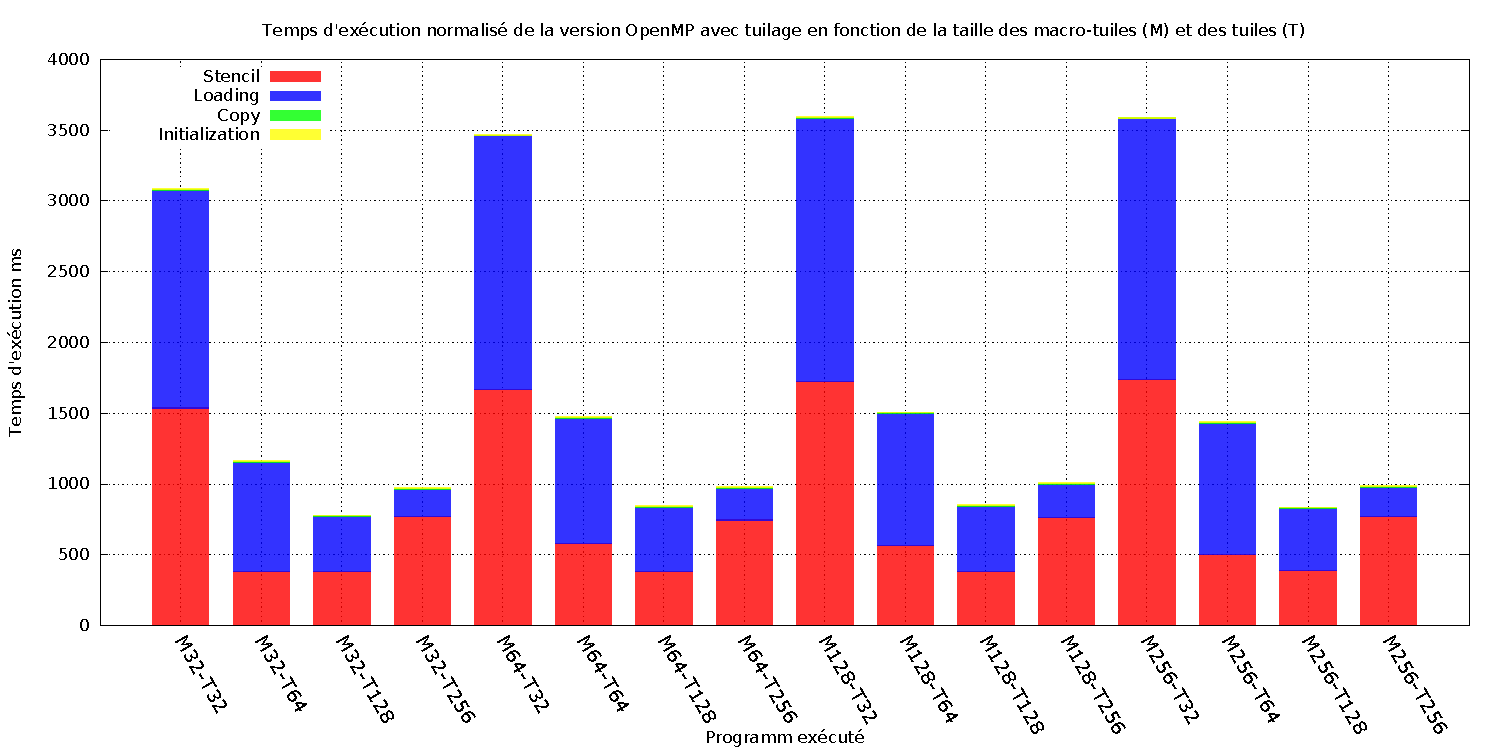
\includegraphics[width=\textwidth]{graph1.pdf}
\end{figure}

Les tailles de tuiles ont été déterminées en fonction de la taille du cache L2. Le nombre de cache-misses pour le cache L2 durant le calcul de stencil (en bleu dans le graphique \ref{graph:comp_tuile_cmiss}) suit la même loi que le temps d'exécution : le pic de performances pour S\_L2 (donc quand il y a le moins de cache-misses) est atteint pour les cas $T128$. En revanche le total des cache-misses (ainsi que S\_L1) est minimal pour les cas $T64$ (en dehors de $M32-T64$), et cette fois-ci la tendance de l'influence de la taille des macro-tuiles est inversée : plus elles sont grandes moins il y a de cache-misses. Ce résultat peut sembler contradictoire avec les temps d'exécution dans le graphique \ref{graph:comp_tuile_time} car plus il y a de cache-misses plus le temps d'exécution est long a priori. Or tous les caches-misses n'induisent pas le même coût en temps : un cache-miss au niveau L3 est beaucoup plus coûteux qu'au niveau L1 car le niveau L1 est plus proche du cœur dans la hiérarchie mémoire. Ainsi la corrélation entre les deux graphiques se situe au niveau des caches L2 dont les cache-misses sont effectivement les moins nombreux pour tous les cas $T128$. 

\begin{figure}[!h]
  \caption{Comparaison des performances en compteurs matériels suivant la taille des tuiles et des macro-tuiles.}
  \label{graph:comp_tuile_cmiss}
  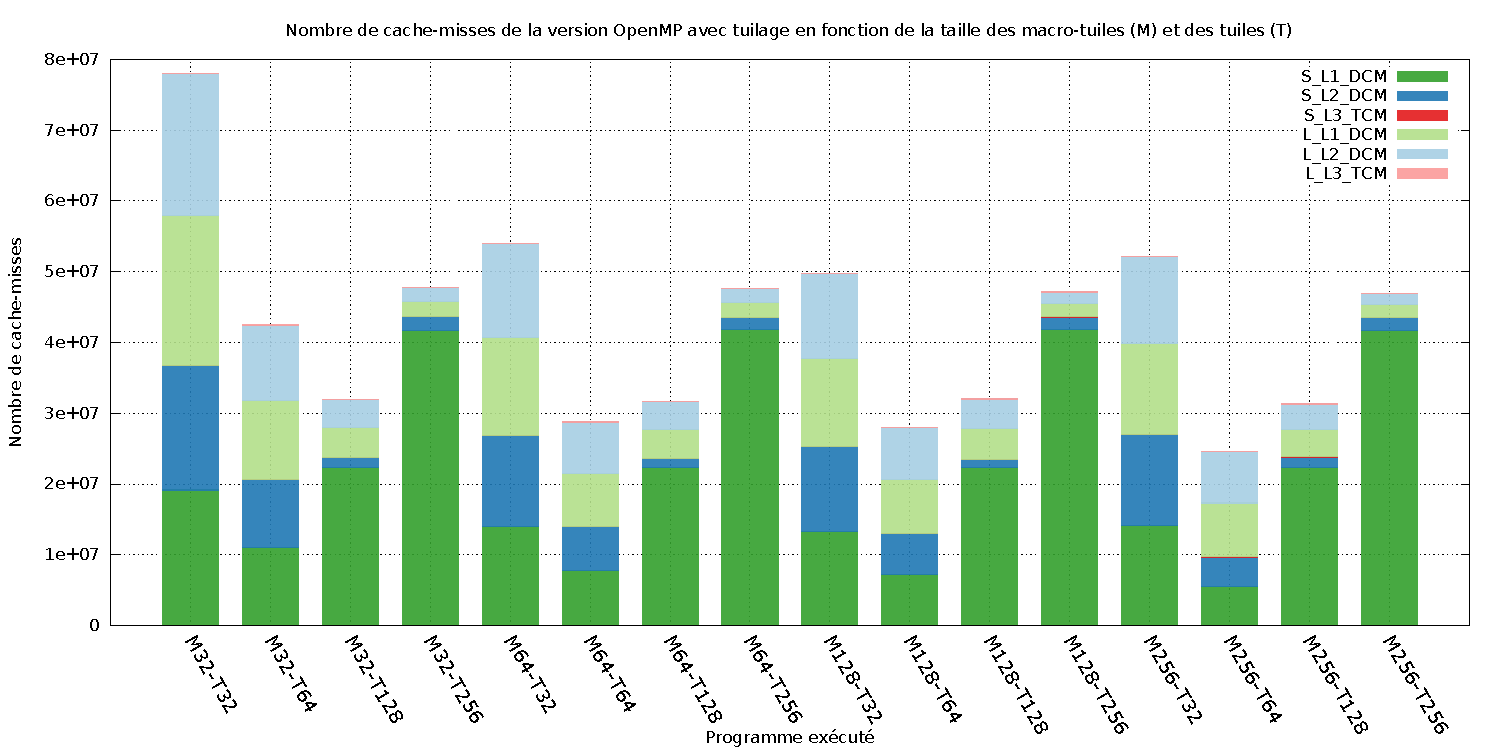
\includegraphics[width=\textwidth]{graph2.pdf}
\end{figure}

Les résultats des compteurs de cache-misses renforcent ainsi l'idée que l'optimisation de la mémoire au sein du cache L2 est très importante pour obtenir des performances. De plus ces résultats expliquent partiellement pourquoi la taille des macro-tuile n'avait pas d'influence sur le temps d'exécution. En effet les cache-misses au niveau L3 (en rouge clair et rouge foncé dans la figure \ref{graph:comp_tuile_cmiss}, non visibles) sont très peu nombreux (de l'ordre de $1\%$ par rapport au L2) quelle que soit la taille des macro-tuiles et donc ils ne modifient pas le temps d'exécution.

Ces résultats sont révélateurs de la complexité des possibilités d'optimisation du DSEL car alors que la taille des macro-tuiles est contrôlable par le DSEL, la taille des tuiles (qui simule la charge de calcul d'une tâche) est gérée par l'utilisateur. Le paradigme utilisé par le DSEL pour le tuilage qui est d'exécuter chaque tâche sur un cœur (une tâche étant l'application d'un stencil sur un élément) n'est donc peut-être pas le plus adapté : il est nécessaire non seulement de gérer la taille des macro-tuiles (car elles peuvent certainement avoir une influence sur d'autres types de problèmes que Jacobi) mais aussi la charge de calcul d'une tâche en les subdivisant ou au contraire en les regroupant, ce qui est difficile à prévoir. Les objectifs de performances évoqués à la section \ref{sec:obj_perf} ne doivent alors pas seulement s'appuyer sur les caractéristiques du L3 mais aussi sur celles du L2 (lorsqu'il s'agit de processeurs centraux).


\subsubsection*{Comparaison des implantations et liens avec le matériel}

Selon la nature du matériel, différentes implantations et méthodes de parallélisation sont adaptées, notamment suivant le nombre de bancs NUMA. Les deux graphiques suivants ont été tracés pour le même cas de Jacobi a priori optimal pour la machine \textsf{Mistral} : $M128-T128$. La figure \ref{graph:comp_temps_mistral10core} regroupe les résultats de plusieurs implantations différentes exécutées sur un seul banc NUMA. La version séquentielle est celle qui nécessite le plus de temps avec la version de parallélisation hiérarchique par banc inadaptée sur un unique banc. Les deux versions de base, avec parallélisation naïve sont les deux implantations les plus performantes et atteignent une accélération de $9.8$, donc presque $10$ fois plus rapide que la version séquentielle soit le pic théorique de performance puisque le banc NUMA dispose de $10$ cœurs. En revanche les versions par tuilage (les trois plus à droite sur la figure \ref{graph:comp_temps_mistral10core}) sont deux fois plus lentes que les versions de base parallélisées naïvement et atteignent une accélération de $4.4$ seulement. Toutefois notons que le coût du calcul du stencil (en rose sur le graphique) est quant à lui similaire et le temps supplémentaire est donc dû au chargement des données des macro-tuiles (en bleu). Ce résultat est prévisible car la parallélisation par tuilage est plutôt adaptée aux processeurs graphiques qui nécessitent explicitement ce chargement en mémoire contrairement aux processeurs centraux tels que dans le cas présent où l'opération de chargement est effectuée automatiquement.

\begin{figure}[!h]
  \caption{Comparaison des performances suivant l'implantation sur un seul banc NUMA.}
  \label{graph:comp_temps_mistral10core}
  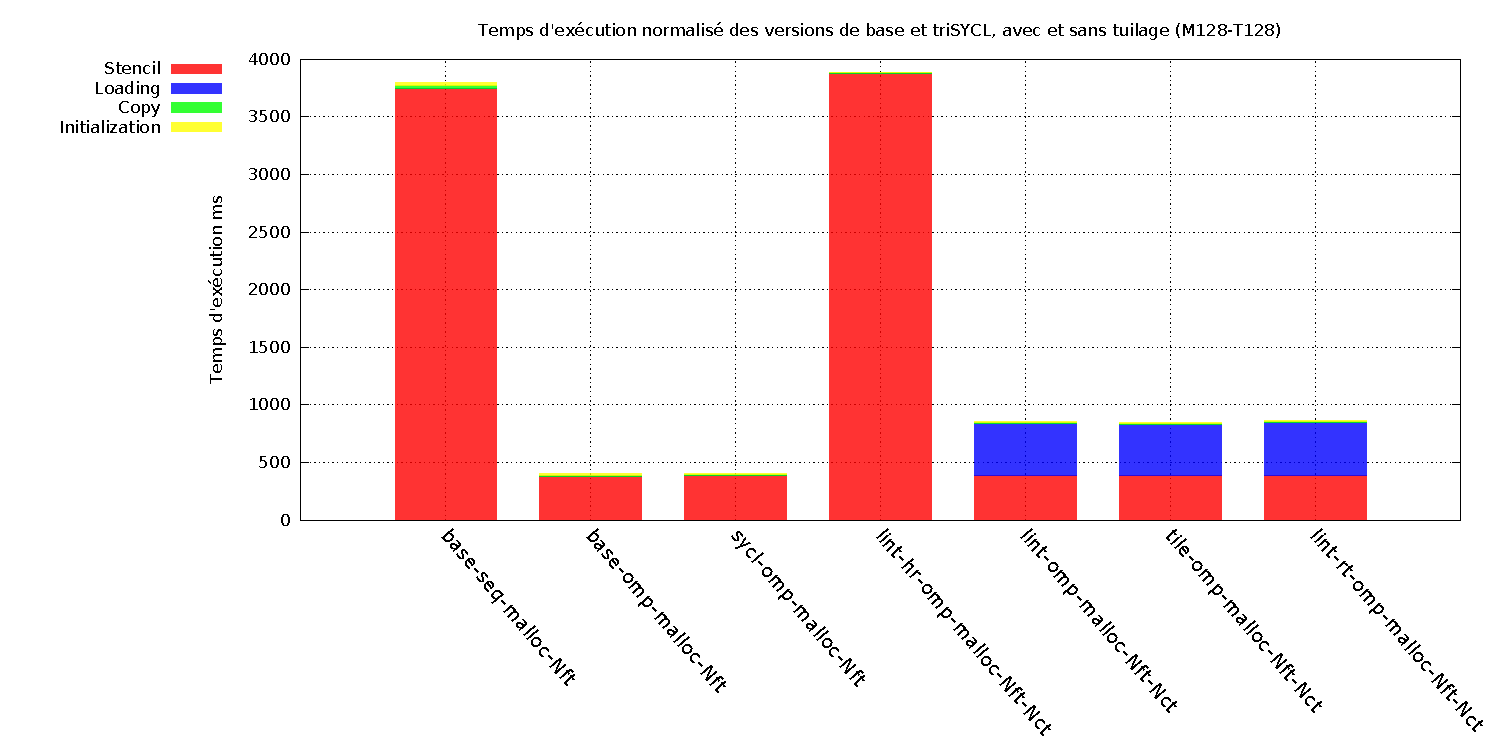
\includegraphics[width=\textwidth]{graph3.pdf}
\end{figure}

L'introduction d'un second banc NUMA pour réaliser les mêmes calculs change radicalement les performances des versions par tuilage et hiérarchiques. Alors que les deux versions de base procurent une accélération de $17$ par rapport à la version séquentielle et restent donc proches de la limite théorique de $20$ (avec deux bancs NUMA, il y a $20$ cœurs disponibles), les trois versions parallélisées par tuilage sont à peine meilleures que la version séquentielle. En effet l'introduction du second banc NUMA provoque des chargements mémoires plus lents à cause de l'interconnexion des deux bancs. La version hiérarchique --- barre centrale dans la figure \ref{graph:comp_temps_mistral20core} --- est légèrement meilleure et atteint une accélération de $1.9$, ce qui est largement en-dessous des performances théoriques. L'introduction d'un plus grand nombre de bancs NUMA a été étudiée avec la machine \textsf{Manumanu} et l'utilisation simultanée de $8$ bancs. La version hiérarchique est alors beaucoup plus bénéfique et rattrape les performances de la parallélisation naïve. En revanche les versions avec tuilage sont alors jusqu'à $10$ fois plus lentes que la version séquentielle et ne sont donc plus adaptées du tout.

\begin{figure}[!h]
  \caption{Comparaison des performances suivant l'implantation sur deux bancs NUMA.}
  \label{graph:comp_temps_mistral20core}
  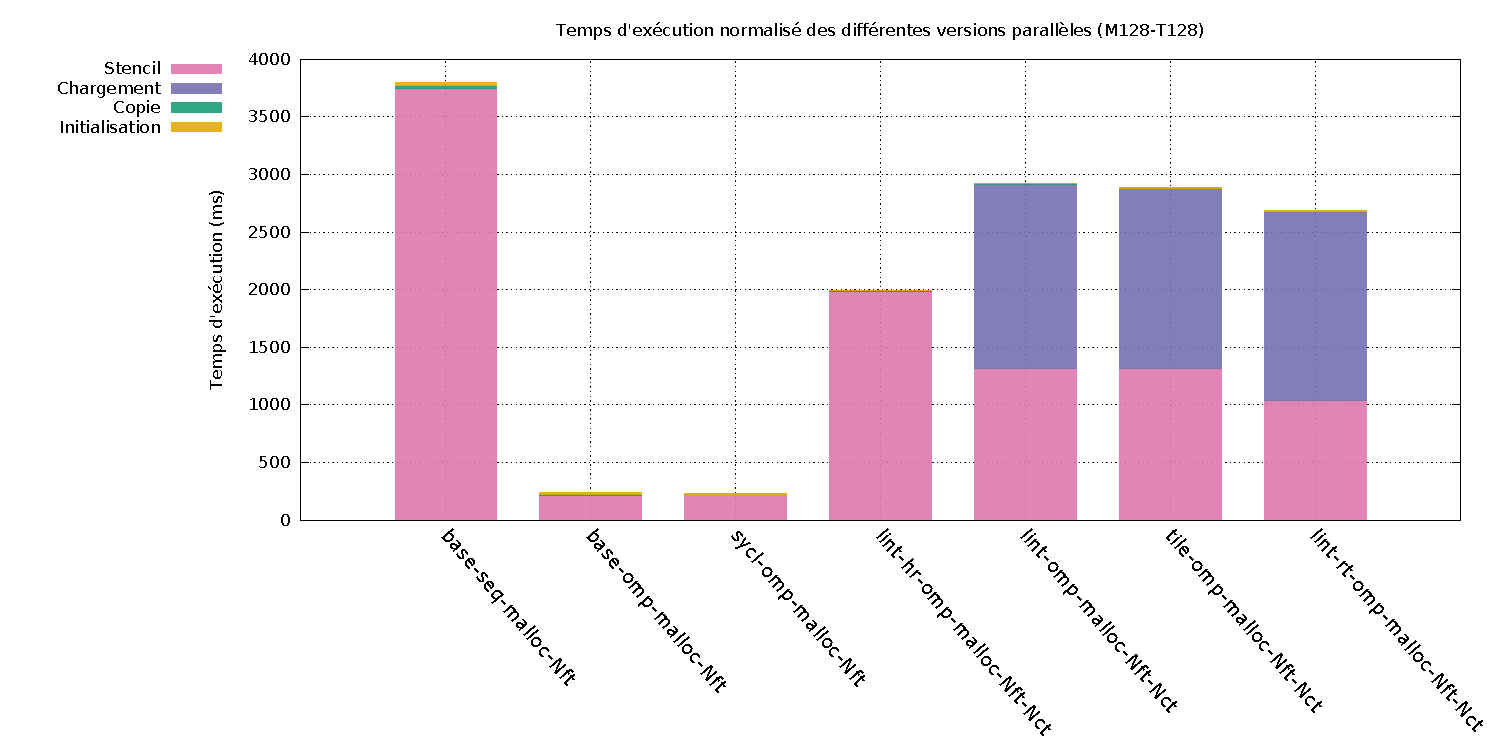
\includegraphics[width=\textwidth]{graph4.pdf}
\end{figure}

La hiérarchisation de la parallélisation a déjà été étudiée dans des travaux tels que \cite{Ths3,Ths4}, il conviendrait alors d'utiliser des techniques similaires pour le DSEL afin d'obtenir des performances raisonnables pour l'utilisation de plusieurs bancs NUMA. Par ailleurs des tests restent à effectuer concernant les cartes graphiques auxquelles est normalement dédiée la parallélisation par tuilage. Cela ne sera toutefois possible qu'avec une autre implantation de \textsf{SYCL} que celle utilisée actuellement, or aucune autre n'est disponible à ce jour\footnote{Une implantation privée est en cours de développement par l'entreprise \textsf{CodePlay}, mais n'est pas encore publiée et sera certainement payante contrairement à \textsf{triSYCL}.}.

Par ailleurs les résultats précédents confirment l'hypothèse que le DSEL n'augmente pas le temps d'exécution puisque les versions utilisant \textsf{triSYCL} ont des performances égales (et même très légèrement meilleures) que les versions de bases (cf les deuxième et troisième barres des deux graphiques précédents, ainsi que les cinquième et sixième, la première étant tout à gauche).

L'évaluation du DSEL a ainsi permis de confirmer certaines hypothèses comme l'influence de la taille des tuiles et la non-influence de l'utilisation d'une bibliothèque comme \textsf{triSYCL}. Toutefois un travail supplémentaire reste à effectuer sur le choix des implantations les plus efficaces notamment dans le cas des machines possédant plusieurs bancs NUMA.
